\begin{frame}
\frametitle{Vector fields}
\begin{itemize}
\item \emph{Vector fields} are functions with multidimensional input and output. 
\item Input is point in space; output is a vector, which we plot as a vector with a tail at the input point. 
\item Examples
\begin{itemize}
  \item Velocity of fluid/air at given point;
  \item Electric force per unit of charge;
  \item Gravitational field;
  %\item Fundamental directions $\textbf{e}_\rho$, $\textbf{e}_\phi$, $\textbf{e}_\theta$, $\textbf{e}_r$
\end{itemize}
\end{itemize}
\end{frame}

\begin{frame}
\frametitle{Coordinate representation of vector fields}

\begin{itemize}
\item In rectangular coordinates a vector field $\textbf{F}$ can
be decomposed along the fundamental directions:
$$
\textbf{F}(x,y,z) = F_1(x,y,z) \textbf{i} + F_2(x,y,z) \textbf{j} + F_3(x,y,z) \textbf{k} \; .
$$
\item For regions in the plane 2-dim vector fields are defined in a similar fashion: as function from subsets of $\mathbb R^2$ to $\RR$.

\item Example: the vector field $\textbf{e}_r$ is given by

\end{itemize}
%
%
$$\textbf{e}_r = \cos\theta\, \textbf{i} +
\sin\theta \,\textbf{j} = \frac{x}{r} \, \textbf{i} +
\frac{y}{r} \, \textbf{j} = \frac{x}{\sqrt{x^2+y^2}} \,
\textbf{i} + \frac{y}{\sqrt{x^2+y^2}} \, \textbf{j}$$
%
and is defined on $\mathbb{R}^2 \setminus \{ (0,0)\}$.
Similarly the vector field $\textbf{e}_{\theta}$ is
%
$$\textbf{e}_\theta = -\sin\theta\, \textbf{i} +
\cos\theta \,\textbf{j} = -\frac{y}{r} \, \textbf{i} +
\frac{x}{r} \, \textbf{j} = -\frac{y}{\sqrt{x^2+y^2}} \,
\textbf{i} + \frac{x}{\sqrt{x^2+y^2}} \, \textbf{j} \; .$$
%
 \begin{center}
\begin{tabular}{cc}
  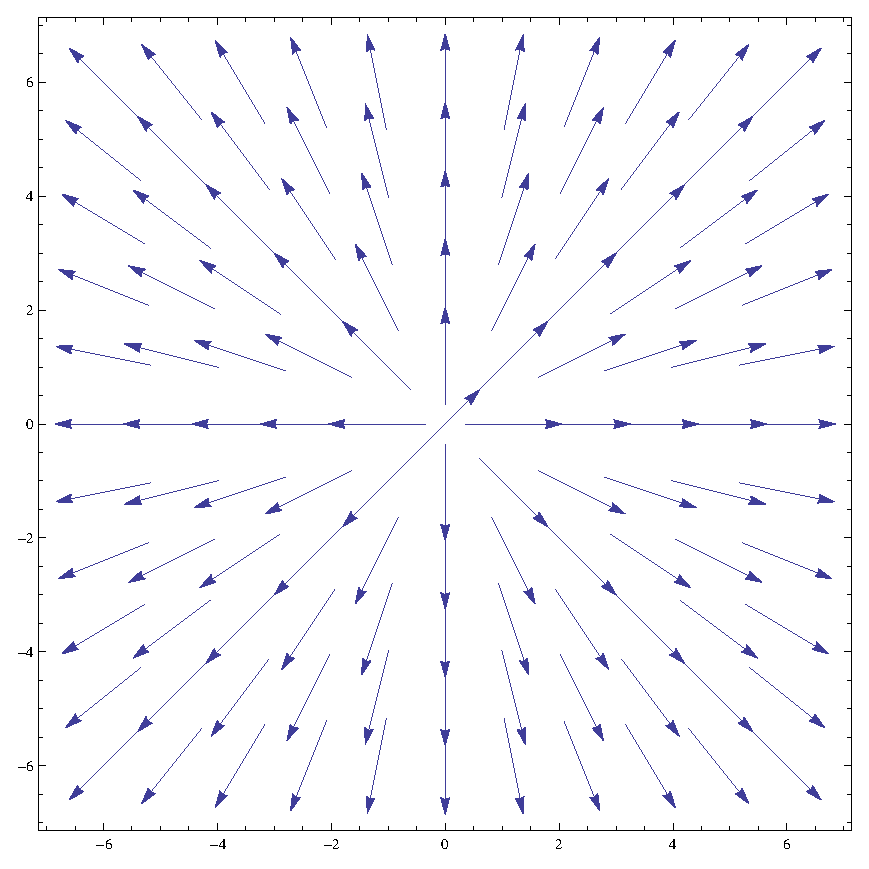
\includegraphics[height=5cm]{../../modules/multivariable-functions/pictures/radial_field.eps}
  &
  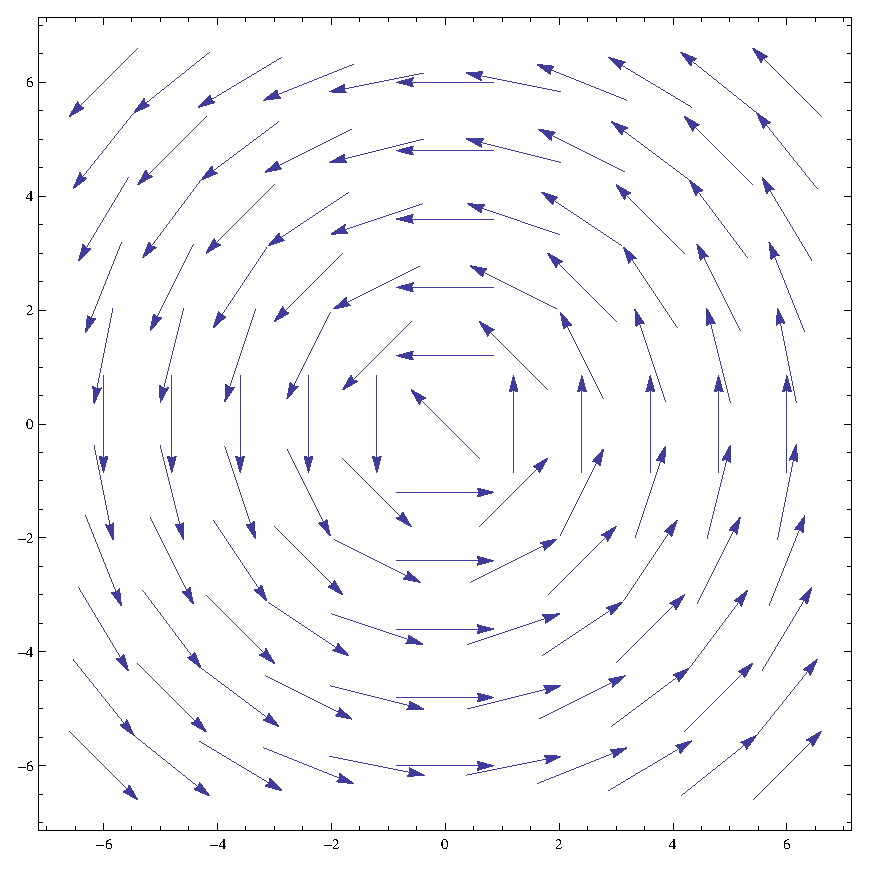
\includegraphics[height=5cm]{../../modules/multivariable-functions/pictures/rotational_field.eps}
  \\
  Radial field $\textbf{e}_r$ & Rotational field
  $\textbf{e}_\theta$
\end{tabular}
\end{center}

The graphical representations of these vector fields makes
it quite clear what would happen to an object forced to move
so that the velocity at each point is given by the value of
the field.

Similar to decomposition in rectangular coordinates
we can decompose a vector field along fundamental vectors
corresponding to other coordinate systems. Things are a bit
trickier, since the fundamental vectors change from
point to point.

In particular, a planar vector field can be written in terms of
$\textbf{e}_r$ and $\textbf{e}_\theta$:
%
$$\textbf{X}(r,\theta) = X_1(r,\theta) \textbf{e}_r\, +
X_2(r,\theta) \textbf{e}_\theta\; .$$
%
For example, if $X(P) = \textbf{i}$, then
%
$$X(r,\theta) = \cos\theta \,\textbf{e}_r\,
-\sin\theta \, \textbf{e}_\theta\; .$$
\end{frame}